\documentclass[NEMO_book]{subfiles}
\begin{document}

% ================================================================
% Chapter ———  Lateral Ocean Physics (LDF)
% ================================================================
\chapter{Lateral Ocean Physics (LDF)}
\label{LDF}
\minitoc


\newpage
$\ $\newline    % force a new ligne


The lateral physics terms in the momentum and tracer equations have been 
described in \S\ref{PE_zdf} and their discrete formulation in \S\ref{TRA_ldf} 
and \S\ref{DYN_ldf}). In this section we further discuss each lateral physics option. 
Choosing one lateral physics scheme means for the user defining, (1) the space 
and time variations of the eddy coefficients ; (2) the direction along which the 
lateral diffusive fluxes are evaluated (model level, geopotential or isopycnal 
surfaces); and (3) the type of operator used (harmonic, or biharmonic operators, 
and for tracers only, eddy induced advection on tracers). These three aspects 
of the lateral diffusion are set through namelist parameters and CPP keys 
(see the \textit{\ngn{nam\_traldf}} and \textit{\ngn{nam\_dynldf}} below). Note
that this chapter describes the default implementation of iso-neutral
tracer mixing, and Griffies's implementation, which is used if
\np{traldf\_grif}=true, is described in Appdx\ref{sec:triad}

%-----------------------------------nam_traldf - nam_dynldf--------------------------------------------
\namdisplay{namtra_ldf} 
\namdisplay{namdyn_ldf} 
%--------------------------------------------------------------------------------------------------------------


% ================================================================
% Lateral Mixing Coefficients
% ================================================================
\section [Lateral Mixing Coefficient (\textit{ldftra}, \textit{ldfdyn})] 
		  {Lateral Mixing Coefficient (\mdl{ldftra}, \mdl{ldfdyn}) }
\label{LDF_coef}


Introducing a space variation in the lateral eddy mixing coefficients changes 
the model core memory requirement, adding up to four extra three-dimensional 
arrays for the geopotential or isopycnal second order operator applied to 
momentum. Six CPP keys control the space variation of eddy coefficients: 
three for momentum and three for tracer. The three choices allow: 
a space variation in the three space directions (\key{traldf\_c3d},  \key{dynldf\_c3d}), 
in the horizontal plane (\key{traldf\_c2d},  \key{dynldf\_c2d}), 
or in the vertical only (\key{traldf\_c1d},  \key{dynldf\_c1d}). 
The default option is a constant value over the whole ocean on both momentum and tracers. 
   
The number of additional arrays that have to be defined and the gridpoint 
position at which they are defined depend on both the space variation chosen 
and the type of operator used. The resulting eddy viscosity and diffusivity 
coefficients can be a function of more than one variable. Changes in the 
computer code when switching from one option to another have been 
minimized by introducing the eddy coefficients as statement functions
(include file \hf{ldftra\_substitute} and \hf{ldfdyn\_substitute}). The functions 
are replaced by their actual meaning during the preprocessing step (CPP). 
The specification of the space variation of the coefficient is made in 
\mdl{ldftra} and \mdl{ldfdyn}, or more precisely in include files 
\textit{traldf\_cNd.h90} and \textit{dynldf\_cNd.h90}, with N=1, 2 or 3. 
The user can modify these include files as he/she wishes. The way the 
mixing coefficient are set in the reference version can be briefly described 
as follows:

\subsubsection{Constant Mixing Coefficients (default option)}
When none of the \textbf{key\_dynldf\_...} and \textbf{key\_traldf\_...} keys are 
defined, a constant value is used over the whole ocean for momentum and 
tracers, which is specified through the \np{rn\_ahm\_0\_lap} and \np{rn\_aht\_0} namelist 
parameters.

\subsubsection{Vertically varying Mixing Coefficients (\key{traldf\_c1d} and \key{dynldf\_c1d})} 
The 1D option is only available when using the $z$-coordinate with full step. 
Indeed in all the other types of vertical coordinate, the depth is a 3D function 
of (\textbf{i},\textbf{j},\textbf{k}) and therefore, introducing depth-dependent 
mixing coefficients will require 3D arrays. In the 1D option, a hyperbolic variation 
of the lateral mixing coefficient is introduced in which the surface value is 
\np{rn\_aht\_0} (\np{rn\_ahm\_0\_lap}), the bottom value is 1/4 of the surface value, 
and the transition takes place around z=300~m with a width of 300~m 
($i.e.$ both the depth and the width of the inflection point are set to 300~m). 
This profile is hard coded in file \hf{traldf\_c1d}, but can be easily modified by users.

\subsubsection{Horizontally Varying Mixing Coefficients (\key{traldf\_c2d} and \key{dynldf\_c2d})}
By default the horizontal variation of the eddy coefficient depends on the local mesh 
size and the type of operator used:
\begin{equation} \label{Eq_title}
  A_l = \left\{     
   \begin{aligned}
         & \frac{\max(e_1,e_2)}{e_{max}} A_o^l  			& \text{for laplacian operator } \\
         & \frac{\max(e_1,e_2)^{3}}{e_{max}^{3}} A_o^l          & \text{for bilaplacian operator } 
   \end{aligned}    \right.
\end{equation}
where $e_{max}$ is the maximum of $e_1$ and $e_2$ taken over the whole masked 
ocean domain, and $A_o^l$ is the \np{rn\_ahm\_0\_lap} (momentum) or \np{rn\_aht\_0} (tracer) 
namelist parameter. This variation is intended to reflect the lesser need for subgrid 
scale eddy mixing where the grid size is smaller in the domain. It was introduced in 
the context of the DYNAMO modelling project \citep{Willebrand_al_PO01}. 
Note that such a grid scale dependance of mixing coefficients significantly increase 
the range of stability of model configurations presenting large changes in grid pacing 
such as global ocean models. Indeed, in such a case, a constant mixing coefficient 
can lead to a blow up of the model due to large coefficient compare to the smallest 
grid size (see \S\ref{STP_forward_imp}), especially when using a bilaplacian operator.

Other formulations can be introduced by the user for a given configuration. 
For example, in the ORCA2 global ocean model (see Configurations), the laplacian 
viscosity operator uses \np{rn\_ahm\_0\_lap}~= 4.10$^4$ m$^2$/s poleward of 20\deg 
north and south and decreases linearly to \np{rn\_aht\_0}~= 2.10$^3$ m$^2$/s 
at the equator \citep{Madec_al_JPO96, Delecluse_Madec_Bk00}. This modification 
can be found in routine \rou{ldf\_dyn\_c2d\_orca} defined in \mdl{ldfdyn\_c2d}. 
Similar modified horizontal variations can be found with the Antarctic or Arctic 
sub-domain options of ORCA2 and ORCA05 (see \&namcfg namelist).

\subsubsection{Space Varying Mixing Coefficients (\key{traldf\_c3d} and \key{dynldf\_c3d})}

The 3D space variation of the mixing coefficient is simply the combination of the 
1D and 2D cases, $i.e.$ a hyperbolic tangent variation with depth associated with 
a grid size dependence of the magnitude of the coefficient. 

\subsubsection{Space and Time Varying Mixing Coefficients}

There are no default specifications of space and time varying mixing coefficient.  One
available case is specific to the ORCA2 and ORCA05 global ocean configurations. It
provides only a tracer mixing coefficient for eddy induced velocity (ORCA2) or both
iso-neutral and eddy induced velocity (ORCA05) that depends on the local growth rate of
baroclinic instability. This specification is actually used when an ORCA key
and both \key{traldf\_eiv} and \key{traldf\_c2d} are defined.

\subsubsection{Smagorinsky viscosity (\key{dynldf\_c3d} and \key{dynldf\_smag})}

The \key{dynldf\_smag} key activates a 3D, time-varying viscosity that depends on the
resolved motions. Following \citep{Smagorinsky_93} the viscosity coefficient is set
proportional to a local deformation rate based on the horizontal shear and tension,
namely:

\begin{equation}
A_{m_{Smag}} = \left(\frac{{\sf CM_{Smag}}}{\pi}\right)^2L^2\vert{D}\vert
\end{equation}

\noindent where the deformation rate $\vert{D}\vert$ is given by 

\begin{equation}
\vert{D}\vert=\sqrt{\left({\frac{\partial{u}} {\partial{x}}}
                         -{\frac{\partial{v}} {\partial{y}}}\right)^2
                 +  \left({\frac{\partial{u}} {\partial{y}}}
                         +{\frac{\partial{v}} {\partial{x}}}\right)^2} 
\end{equation}

\noindent and $L$ is the local gridscale given by:

\begin{equation}
L^2 = \frac{2{e_1}^2 {e_2}^2}{\left ( {e_1}^2 + {e_2}^2 \right )}
\end{equation}

\citep{Griffies_Hallberg_MWR00} suggest values in the range 2.2 to 4.0 of the coefficient
$\sf CM_{Smag}$ for oceanic flows. This value is set via the \np{rn\_cmsmag\_1} namelist
parameter. An additional parameter: \np{rn\_cmsh} is included in NEMO for experimenting
with the contribution of the shear term. A value of 1.0 (the default) calculates the
deformation rate as above; a value of 0.0 will discard the shear term entirely.

For numerical stability, the calculated viscosity is bounded according to the following:

\begin{equation}
{\rm MIN}\left ({ L^2\over {8\Delta{t}}}, rn\_ahm\_m\_lap\right ) \geq A_{m_{Smag}} 
                                                                  \geq rn\_ahm\_0\_lap
\end{equation}

\noindent with both parameters for the upper and lower bounds being provided via the
indicated namelist parameters.

\bigskip When $ln\_dynldf\_bilap = .true.$, a biharmonic version of the Smagorinsky
viscosity is also available which sets a coefficient for the biharmonic viscosity as:

\begin{equation}
B_{m_{Smag}} = - \left(\frac{{\sf CM_{bSmag}}}{\pi}\right)^2 {L^4\over 8}\vert{D}\vert
\end{equation}

\noindent which is bounded according to:

\begin{equation}
{\rm MAX}\left (-{ L^4\over {64\Delta{t}}}, rn\_ahm\_m\_blp\right ) \leq B_{m_{Smag}} 
                                                                    \leq rn\_ahm\_0\_blp
\end{equation}

\noindent Note the reversal of the inequalities here because NEMO requires the biharmonic
coefficients as negative numbers. $\sf CM_{bSmag}$ is set via the \np{rn\_cmsmag\_2}
namelist parameter and the bounding values have corresponding entries in the namelist too.

\bigskip The current implementation in NEMO also allows for 3D, time-varying diffusivities
to be set using the Smagorinsky approach. Users should note that this option is not
recommended for many applications since diffusivities will tend to be largest near
boundaries (where shears are greatest) leading to spurious upwellings
(\citep{Griffies_Bk04}, chapter 18.3.4). Nevertheless the option is there for those
wishing to experiment. This choice requires both \key{traldf\_c3d} and \key{traldf\_smag}
and uses the \np{rn\_chsmag} (${\sf CH_{Smag}}$), \np{rn\_smsh} and \np{rn\_aht\_m}
namelist parameters in an analogous way to \np{rn\_cmsmag\_1}, \np{rn\_cmsh} and
\np{rn\_ahm\_m\_lap} (see above) to set the diffusion coefficient:

\begin{equation}
A_{h_{Smag}} = \left(\frac{{\sf CH_{Smag}}}{\pi}\right)^2L^2\vert{D}\vert
\end{equation}

 
For numerical stability, the calculated diffusivity is bounded according to the following:

\begin{equation}
{\rm MIN}\left ({ L^2\over {8\Delta{t}}}, rn\_aht\_m\right ) \geq A_{h_{Smag}} 
                                                             \geq rn\_aht\_0
\end{equation}



$\ $\newline    % force a new ligne

The following points are relevant when the eddy coefficient varies spatially:

(1) the momentum diffusion operator acting along model level surfaces is 
written in terms of curl and divergent components of the horizontal current 
(see \S\ref{PE_ldf}). Although the eddy coefficient could be set to different values 
in these two terms, this option is not currently available. 

(2) with an horizontally varying viscosity, the quadratic integral constraints 
on enstrophy and on the square of the horizontal divergence for operators 
acting along model-surfaces are no longer satisfied 
(Appendix~\ref{Apdx_dynldf_properties}).

(3) for isopycnal diffusion on momentum or tracers, an additional purely 
horizontal background diffusion with uniform coefficient can be added by 
setting a non zero value of \np{rn\_ahmb\_0} or \np{rn\_ahtb\_0}, a background horizontal 
eddy viscosity or diffusivity coefficient (namelist parameters whose default 
values are $0$). However, the technique used to compute the isopycnal 
slopes is intended to get rid of such a background diffusion, since it introduces 
spurious diapycnal diffusion (see \S\ref{LDF_slp}).

(4) when an eddy induced advection term is used (\key{traldf\_eiv}), $A^{eiv}$, 
the eddy induced coefficient has to be defined. Its space variations are controlled 
by the same CPP variable as for the eddy diffusivity coefficient ($i.e.$ 
\textbf{key\_traldf\_cNd}). 

(5) the eddy coefficient associated with a biharmonic operator must be set to a \emph{negative} value.

(6) it is possible to use both the laplacian and biharmonic operators concurrently.

(7) it is possible to run without explicit lateral diffusion on momentum (\np{ln\_dynldf\_lap} = 
\np{ln\_dynldf\_bilap} = false). This is recommended when using the UBS advection 
scheme on momentum (\np{ln\_dynadv\_ubs} = true, see \ref{DYN_adv_ubs}) 
and can be useful for testing purposes.

% ================================================================
% Direction of lateral Mixing
% ================================================================
\section  [Direction of Lateral Mixing (\textit{ldfslp})]
		{Direction of Lateral Mixing (\mdl{ldfslp})}
\label{LDF_slp}

%%%
\gmcomment{  we should emphasize here that the implementation is a rather old one. 
Better work can be achieved by using \citet{Griffies_al_JPO98, Griffies_Bk04} iso-neutral scheme. }

A direction for lateral mixing has to be defined when the desired operator does 
not act along the model levels. This occurs when $(a)$ horizontal mixing is 
required on tracer or momentum (\np{ln\_traldf\_hor} or \np{ln\_dynldf\_hor}) 
in $s$- or mixed $s$-$z$- coordinates, and $(b)$ isoneutral mixing is required 
whatever the vertical coordinate is. This direction of mixing is defined by its 
slopes in the \textbf{i}- and \textbf{j}-directions at the face of the cell of the 
quantity to be diffused. For a tracer, this leads to the following four slopes : 
$r_{1u}$, $r_{1w}$, $r_{2v}$, $r_{2w}$ (see \eqref{Eq_tra_ldf_iso}), while 
for momentum the slopes are  $r_{1t}$, $r_{1uw}$, $r_{2f}$, $r_{2uw}$ for 
$u$ and  $r_{1f}$, $r_{1vw}$, $r_{2t}$, $r_{2vw}$ for $v$. 

%gm% add here afigure of the slope in i-direction

\subsection{slopes for tracer geopotential mixing in the $s$-coordinate}

In $s$-coordinates, geopotential mixing ($i.e.$ horizontal mixing) $r_1$ and 
$r_2$ are the slopes between the geopotential and computational surfaces. 
Their discrete formulation is found by locally solving \eqref{Eq_tra_ldf_iso} 
when the diffusive fluxes in the three directions are set to zero and $T$ is 
assumed to be horizontally uniform, $i.e.$ a linear function of $z_T$, the 
depth of a $T$-point. 
%gm { Steven : My version is obviously wrong since I'm left with an arbitrary constant which is the local vertical temperature gradient}

\begin{equation} \label{Eq_ldfslp_geo}
\begin{aligned}
 r_{1u} &= \frac{e_{3u}}{ \left( e_{1u}\;\overline{\overline{e_{3w}}}^{\,i+1/2,\,k} \right)}
 			  \;\delta_{i+1/2}[z_t] 
 		&\approx \frac{1}{e_{1u}}\; \delta_{i+1/2}[z_t] 
\\
 r_{2v} &= \frac{e_{3v}}{\left( e_{2v}\;\overline{\overline{e_{3w}}}^{\,j+1/2,\,k} \right)} 
 			  \;\delta_{j+1/2} [z_t] 
		&\approx \frac{1}{e_{2v}}\; \delta_{j+1/2}[z_t] 
\\
 r_{1w} &= \frac{1}{e_{1w}}\;\overline{\overline{\delta_{i+1/2}[z_t]}}^{\,i,\,k+1/2}
 		&\approx \frac{1}{e_{1w}}\; \delta_{i+1/2}[z_{uw}] 
 \\
 r_{2w} &= \frac{1}{e_{2w}}\;\overline{\overline{\delta_{j+1/2}[z_t]}}^{\,j,\,k+1/2}
		&\approx \frac{1}{e_{2w}}\; \delta_{j+1/2}[z_{vw}] 
 \\
\end{aligned}
\end{equation}

%gm%  caution I'm not sure the simplification was a good idea! 

These slopes are computed once in \rou{ldfslp\_init} when \np{ln\_sco}=True, 
and either \np{ln\_traldf\_hor}=True or \np{ln\_dynldf\_hor}=True. 

\subsection{Slopes for tracer iso-neutral mixing}\label{LDF_slp_iso}
In iso-neutral mixing  $r_1$ and $r_2$ are the slopes between the iso-neutral 
and computational surfaces. Their formulation does not depend on the vertical 
coordinate used. Their discrete formulation is found using the fact that the 
diffusive fluxes of locally referenced potential density ($i.e.$ $in situ$ density) 
vanish. So, substituting $T$ by $\rho$ in \eqref{Eq_tra_ldf_iso} and setting the 
diffusive fluxes in the three directions to zero leads to the following definition for 
the neutral slopes:

\begin{equation} \label{Eq_ldfslp_iso}
\begin{split}
 r_{1u} &= \frac{e_{3u}}{e_{1u}}\; \frac{\delta_{i+1/2}[\rho]}
 								{\overline{\overline{\delta_{k+1/2}[\rho]}}^{\,i+1/2,\,k}}
\\
 r_{2v} &= \frac{e_{3v}}{e_{2v}}\; \frac{\delta_{j+1/2}\left[\rho \right]}
 								{\overline{\overline{\delta_{k+1/2}[\rho]}}^{\,j+1/2,\,k}}
\\
 r_{1w} &= \frac{e_{3w}}{e_{1w}}\; 
 			\frac{\overline{\overline{\delta_{i+1/2}[\rho]}}^{\,i,\,k+1/2}}
				 {\delta_{k+1/2}[\rho]}
\\
 r_{2w} &= \frac{e_{3w}}{e_{2w}}\; 
 			\frac{\overline{\overline{\delta_{j+1/2}[\rho]}}^{\,j,\,k+1/2}}
				 {\delta_{k+1/2}[\rho]}
\\
\end{split}
\end{equation}

%gm% rewrite this as the explanation is not very clear !!!
%In practice, \eqref{Eq_ldfslp_iso} is of little help in evaluating the neutral surface slopes. Indeed, for an unsimplified equation of state, the density has a strong dependancy on pressure (here approximated as the depth), therefore applying \eqref{Eq_ldfslp_iso} using the $in situ$ density, $\rho$, computed at T-points leads to a flattening of slopes as the depth increases. This is due to the strong increase of the $in situ$ density with depth. 

%By definition, neutral surfaces are tangent to the local $in situ$ density \citep{McDougall1987}, therefore in \eqref{Eq_ldfslp_iso}, all the derivatives have to be evaluated at the same local pressure (which in decibars is approximated by the depth in meters).

%In the $z$-coordinate, the derivative of the  \eqref{Eq_ldfslp_iso} numerator is evaluated at the same depth \nocite{as what?} ($T$-level, which is the same as the $u$- and $v$-levels), so  the $in situ$ density can be used for its evaluation. 

As the mixing is performed along neutral surfaces, the gradient of $\rho$ in 
\eqref{Eq_ldfslp_iso} has to be evaluated at the same local pressure (which, 
in decibars, is approximated by the depth in meters in the model). Therefore 
\eqref{Eq_ldfslp_iso} cannot be used as such, but further transformation is 
needed depending on the vertical coordinate used:

\begin{description}

\item[$z$-coordinate with full step : ] in \eqref{Eq_ldfslp_iso} the densities 
appearing in the $i$ and $j$ derivatives  are taken at the same depth, thus 
the $in situ$ density can be used. This is not the case for the vertical 
derivatives: $\delta_{k+1/2}[\rho]$ is replaced by $-\rho N^2/g$, where $N^2$ 
is the local Brunt-Vais\"{a}l\"{a} frequency evaluated following 
\citet{McDougall1987} (see \S\ref{TRA_bn2}). 

\item[$z$-coordinate with partial step : ] this case is identical to the full step 
case except that at partial step level, the \emph{horizontal} density gradient 
is evaluated as described in \S\ref{TRA_zpshde}.

\item[$s$- or hybrid $s$-$z$- coordinate : ] in the current release of \NEMO, 
iso-neutral mixing is only employed for $s$-coordinates if the
Griffies scheme is used (\np{traldf\_grif}=true; see Appdx \ref{sec:triad}). 
In other words, iso-neutral mixing will only be accurately represented with a 
linear equation of state (\np{nn\_eos}=1 or 2). In the case of a "true" equation 
of state, the evaluation of $i$ and $j$ derivatives in \eqref{Eq_ldfslp_iso} 
will include a pressure dependent part, leading to the wrong evaluation of 
the neutral slopes.

%gm% 
Note: The solution for $s$-coordinate passes trough the use of different 
(and better) expression for the constraint on iso-neutral fluxes. Following 
\citet{Griffies_Bk04}, instead of specifying directly that there is a zero neutral 
diffusive flux of locally referenced potential density, we stay in the $T$-$S$ 
plane and consider the balance between the neutral direction diffusive fluxes 
of potential temperature and salinity:
\begin{equation}
\alpha \ \textbf{F}(T) = \beta \ \textbf{F}(S)
\end{equation}
%gm{  where vector F is ....}

This constraint leads to the following definition for the slopes:

\begin{equation} \label{Eq_ldfslp_iso2}
\begin{split}
 r_{1u} &= \frac{e_{3u}}{e_{1u}}\; \frac
 		{\alpha_u \;\delta_{i+1/2}[T] - \beta_u \;\delta_{i+1/2}[S]}
		{\alpha_u \;\overline{\overline{\delta_{k+1/2}[T]}}^{\,i+1/2,\,k}
		 -\beta_u  \;\overline{\overline{\delta_{k+1/2}[S]}}^{\,i+1/2,\,k} }
\\
 r_{2v} &= \frac{e_{3v}}{e_{2v}}\; \frac
 		{\alpha_v \;\delta_{j+1/2}[T] - \beta_v \;\delta_{j+1/2}[S]}
		{\alpha_v \;\overline{\overline{\delta_{k+1/2}[T]}}^{\,j+1/2,\,k}
		 -\beta_v  \;\overline{\overline{\delta_{k+1/2}[S]}}^{\,j+1/2,\,k} }
\\
 r_{1w} &= \frac{e_{3w}}{e_{1w}}\; \frac
		{\alpha_w \;\overline{\overline{\delta_{i+1/2}[T]}}^{\,i,\,k+1/2}
		 -\beta_w  \;\overline{\overline{\delta_{i+1/2}[S]}}^{\,i,\,k+1/2} }
 		{\alpha_w \;\delta_{k+1/2}[T] - \beta_w \;\delta_{k+1/2}[S]}
\\
 r_{2w} &= \frac{e_{3w}}{e_{2w}}\; \frac
		{\alpha_w \;\overline{\overline{\delta_{j+1/2}[T]}}^{\,j,\,k+1/2}
		 -\beta_w  \;\overline{\overline{\delta_{j+1/2}[S]}}^{\,j,\,k+1/2} }
 		{\alpha_w \;\delta_{k+1/2}[T] - \beta_w \;\delta_{k+1/2}[S]}
\\
\end{split}
\end{equation}
where $\alpha$ and $\beta$, the thermal expansion and saline contraction 
coefficients introduced in \S\ref{TRA_bn2}, have to be evaluated at the three 
velocity points. In order to save computation time, they should be approximated 
by the mean of their values at $T$-points (for example in the case of $\alpha$:  
$\alpha_u=\overline{\alpha_T}^{i+1/2}$,  $\alpha_v=\overline{\alpha_T}^{j+1/2}$ 
and $\alpha_w=\overline{\alpha_T}^{k+1/2}$).

Note that such a formulation could be also used in the $z$-coordinate and 
$z$-coordinate with partial steps cases.

\end{description}

This implementation is a rather old one. It is similar to the one
proposed by Cox [1987], except for the background horizontal
diffusion. Indeed, the Cox implementation of isopycnal diffusion in
GFDL-type models requires a minimum background horizontal diffusion
for numerical stability reasons.  To overcome this problem, several
techniques have been proposed in which the numerical schemes of the
ocean model are modified \citep{Weaver_Eby_JPO97,
  Griffies_al_JPO98}. Griffies's scheme is now available in \NEMO if
\np{traldf\_grif\_iso} is set true; see Appdx \ref{sec:triad}. Here,
another strategy is presented \citep{Lazar_PhD97}: a local
filtering of the iso-neutral slopes (made on 9 grid-points) prevents
the development of grid point noise generated by the iso-neutral
diffusion operator (Fig.~\ref{Fig_LDF_ZDF1}). This allows an
iso-neutral diffusion scheme without additional background horizontal
mixing. This technique can be viewed as a diffusion operator that acts
along large-scale (2~$\Delta$x) \gmcomment{2deltax doesnt seem very
  large scale} iso-neutral surfaces. The diapycnal diffusion required
for numerical stability is thus minimized and its net effect on the
flow is quite small when compared to the effect of an horizontal
background mixing.

Nevertheless, this iso-neutral operator does not ensure that variance cannot increase, 
contrary to the \citet{Griffies_al_JPO98} operator which has that property. 

%>>>>>>>>>>>>>>>>>>>>>>>>>>>>
\begin{figure}[!ht]      \begin{center}
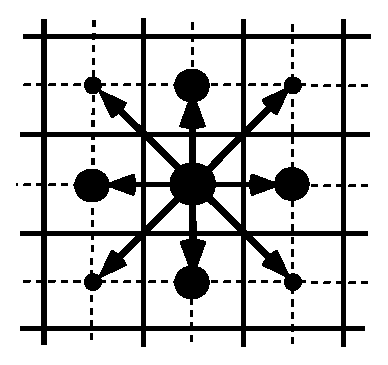
\includegraphics[width=0.70\textwidth]{Fig_LDF_ZDF1}
\caption {    \label{Fig_LDF_ZDF1}
averaging procedure for isopycnal slope computation.}
\end{center}    \end{figure}
%>>>>>>>>>>>>>>>>>>>>>>>>>>>>

%There are three additional questions about the slope calculation. 
%First the expression for the rotation tensor has been obtain assuming the "small slope" approximation, so a bound has to be imposed on slopes. 
%Second, numerical stability issues also require a bound on slopes. 
%Third, the question of boundary condition specified on slopes...

%from griffies: chapter 13.1....



% In addition and also for numerical stability reasons \citep{Cox1987, Griffies_Bk04}, 
% the slopes are bounded by $1/100$ everywhere. This limit is decreasing linearly 
% to zero fom $70$ meters depth and the surface (the fact that the eddies "feel" the 
% surface motivates this flattening of isopycnals near the surface).

For numerical stability reasons \citep{Cox1987, Griffies_Bk04}, the slopes must also 
be bounded by $1/100$ everywhere. This constraint is applied in a piecewise linear 
fashion, increasing from zero at the surface to $1/100$ at $70$ metres and thereafter 
decreasing to zero at the bottom of the ocean. (the fact that the eddies "feel" the 
surface motivates this flattening of isopycnals near the surface).

%>>>>>>>>>>>>>>>>>>>>>>>>>>>>
\begin{figure}[!ht]     \begin{center}
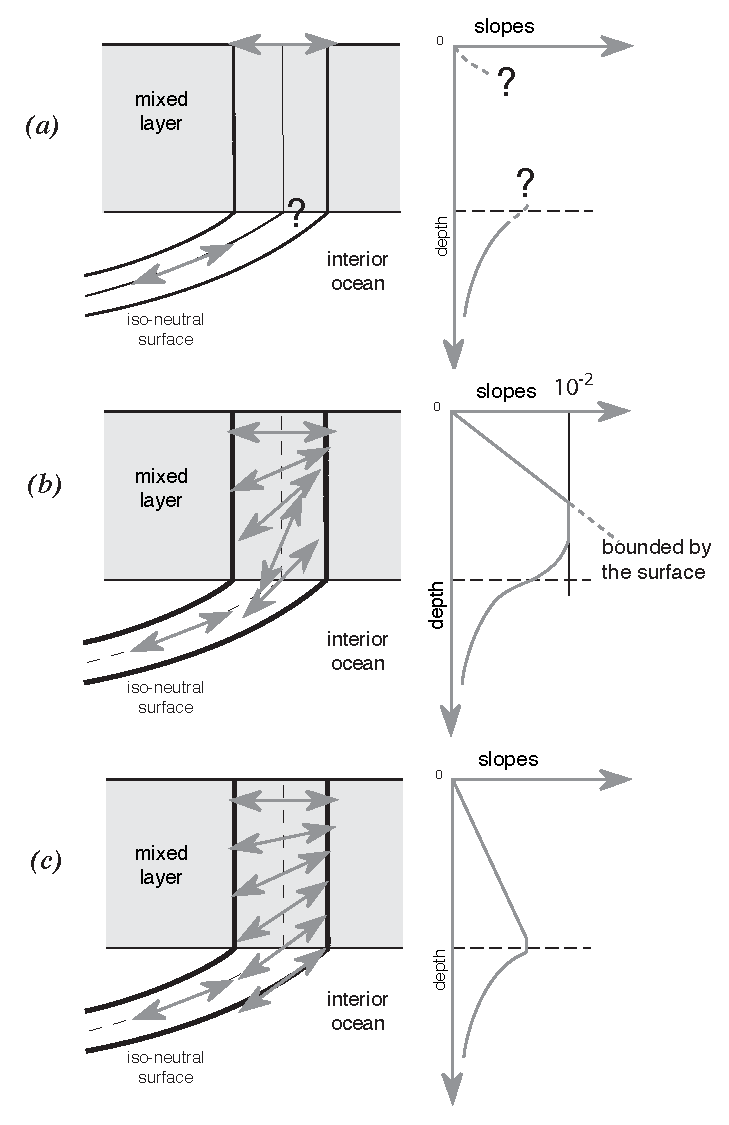
\includegraphics[width=0.70\textwidth]{Fig_eiv_slp}
\caption {     \label{Fig_eiv_slp}
Vertical profile of the slope used for lateral mixing in the mixed layer : 
\textit{(a)} in the real ocean the slope is the iso-neutral slope in the ocean interior, 
which has to be adjusted at the surface boundary (i.e. it must tend to zero at the 
surface since there is no mixing across the air-sea interface: wall boundary 
condition). Nevertheless, the profile between the surface zero value and the interior 
iso-neutral one is unknown, and especially the value at the base of the mixed layer ; 
\textit{(b)} profile of slope using a linear tapering of the slope near the surface and 
imposing a maximum slope of 1/100 ; \textit{(c)} profile of slope actually used in 
\NEMO: a linear decrease of the slope from zero at the surface to its ocean interior 
value computed just below the mixed layer. Note the huge change in the slope at the 
base of the mixed layer between  \textit{(b)}  and \textit{(c)}.}
\end{center}   \end{figure}
%>>>>>>>>>>>>>>>>>>>>>>>>>>>>

\colorbox{yellow}{add here a discussion about the flattening of the slopes, vs  tapering the coefficient.}

\subsection{slopes for momentum iso-neutral mixing}

The iso-neutral diffusion operator on momentum is the same as the one used on 
tracers but applied to each component of the velocity separately (see 
\eqref{Eq_dyn_ldf_iso} in section~\ref{DYN_ldf_iso}). The slopes between the 
surface along which the diffusion operator acts and the surface of computation 
($z$- or $s$-surfaces) are defined at $T$-, $f$-, and \textit{uw}- points for the 
$u$-component, and $T$-, $f$- and \textit{vw}- points for the $v$-component. 
They are computed from the slopes used for tracer diffusion, $i.e.$ 
\eqref{Eq_ldfslp_geo} and \eqref{Eq_ldfslp_iso} :

\begin{equation} \label{Eq_ldfslp_dyn}
\begin{aligned}
&r_{1t}\ \ = \overline{r_{1u}}^{\,i}       &&&    r_{1f}\ \ &= \overline{r_{1u}}^{\,i+1/2} \\
&r_{2f} \ \ = \overline{r_{2v}}^{\,j+1/2} &&& 	r_{2t}\ &= \overline{r_{2v}}^{\,j} \\
&r_{1uw}  = \overline{r_{1w}}^{\,i+1/2} &&\ \ \text{and} \ \ &   r_{1vw}&= \overline{r_{1w}}^{\,j+1/2} \\
&r_{2uw}= \overline{r_{2w}}^{\,j+1/2} &&&         r_{2vw}&= \overline{r_{2w}}^{\,j+1/2}\\
\end{aligned}
\end{equation}

The major issue remaining is in the specification of the boundary conditions. 
The same boundary conditions are chosen as those used for lateral 
diffusion along model level surfaces, i.e. using the shear computed along 
the model levels and with no additional friction at the ocean bottom (see 
\S\ref{LBC_coast}).


% ================================================================
% Eddy Induced Mixing
% ================================================================
\section  [Eddy Induced Velocity (\textit{traadv\_eiv}, \textit{ldfeiv})]
		{Eddy Induced Velocity (\mdl{traadv\_eiv}, \mdl{ldfeiv})}
\label{LDF_eiv}

When Gent and McWilliams [1990] diffusion is used (\key{traldf\_eiv} defined), 
an eddy induced tracer advection term is added, the formulation of which 
depends on the slopes of iso-neutral surfaces. Contrary to the case of iso-neutral 
mixing, the slopes used here are referenced to the geopotential surfaces, $i.e.$ 
\eqref{Eq_ldfslp_geo} is used in $z$-coordinates, and the sum \eqref{Eq_ldfslp_geo}  
+ \eqref{Eq_ldfslp_iso} in $s$-coordinates. The eddy induced velocity is given by: 
\begin{equation} \label{Eq_ldfeiv}
\begin{split}
 u^* & = \frac{1}{e_{2u}e_{3u}}\; \delta_k \left[e_{2u} \, A_{uw}^{eiv} \; \overline{r_{1w}}^{\,i+1/2} \right]\\
v^* & = \frac{1}{e_{1u}e_{3v}}\; \delta_k \left[e_{1v} \, A_{vw}^{eiv} \; \overline{r_{2w}}^{\,j+1/2} \right]\\
w^* & = \frac{1}{e_{1w}e_{2w}}\; \left\{ \delta_i \left[e_{2u} \, A_{uw}^{eiv} \; \overline{r_{1w}}^{\,i+1/2} \right] + \delta_j \left[e_{1v} \, A_{vw}^{eiv} \; \overline{r_{2w}}^{\,j+1/2} \right] \right\} \\
\end{split}
\end{equation}
where $A^{eiv}$ is the eddy induced velocity coefficient whose value is set 
through \np{rn\_aeiv}, a \textit{nam\_traldf} namelist parameter. 
The three components of the eddy induced velocity are computed and add 
to the eulerian velocity in \mdl{traadv\_eiv}. This has been preferred to a 
separate computation of the advective trends associated with the eiv velocity, 
since it allows us to take advantage of all the advection schemes offered for 
the tracers (see \S\ref{TRA_adv}) and not just the $2^{nd}$ order advection 
scheme as in previous releases of OPA \citep{Madec1998}. This is particularly 
useful for passive tracers where \emph{positivity} of the advection scheme is 
of paramount importance. 

At the surface, lateral and bottom boundaries, the eddy induced velocity, 
and thus the advective eddy fluxes of heat and salt, are set to zero. 





\end{document}
